In einem Abstand von circa 4,5 m vom Kollisionspunkt deckt das EMCal einen Azimuthalwinkelbereich von $\phi=107^{\circ}$ und einen Pseudorapiditätsbreich von $ |\eta| \leq 0\,7$ ab.
%Aufgrund von Detektormaterial und Trägerstrukturen zwischen dem primären Vertex und dem EMCal können Teilchen abgelenkt werden oder Photonen in ein Elektron-Positron-Paar konvertieren.
%Die Konvertierung von Photonen ist besonders zu beachten, da in dieser Analyse $\pi^{0}$, welche in zwei Photonen zerfallen, rekonstruiert werden.
Das EMCal besteht aus zwölf Supermodulen, zehn normal großen und zwei kleineren.
Ein normal großes Supermodul besteht aus $24\times48$ Zellen, ein kleineres Supermodul aus $8\times48$ Zellen.
Insgesamt hat das EMCal also 12288 Zellen, die hauptsächlich Photonen, Elektronen und Positronen detektieren und dabei die Energie dieser Teilchen messen.
%Ein normal großes Supermodul unterteilt sich in 24  Streifenmodule, welche wiederum aus 12 Modulen zusammengesetzt sind.
%Jedes Modul beinhaltet 4 Zellen, womit das EMCal aus insgesamt 12288 Zellen besteht.
%Die Zellen sind für das Detektieren und Messen der Energie von hauptsächlich Photonen, Elektronen und Positronen verantwortlich.
Eine einzelne Zelle besteht aus abwechselnd 77 Szintillator- und 76 Bleischichten.
In den Bleischichten entstehen elektromagnetische Schauer, indem eintreffende Photonen durch Paarerzeugung in ein Elektron und ein Positron konvertieren, die wiederum durch Bremsstrahlung weitere Photonen abstrahlen.
Die Szintillatoren werden durch die Photonen angeregt und geben ein messbares Lichtsignal ab.
Alle Szintillatorschichten einer Zelle sind über einen Lichtleiter mit einem Photomultiplier verbunden.
Der Photomultiplier wandelt das Lichtsignal in ein elektrisches Signal um, das proportional zur detektierten Energie der Zelle ist.
\newline
Jeder elektromagnetische Schauer besitzt eine gewisse Ausdehnung, die über den Moli\`ere-Radius $R_{\text{M}}$ definiert ist.
Der Moli\`ere-Radius gibt den Radius passend zu einem Zylinder an, in dem 90\% der gesamten Energie eines Schauers vom Detektor gemessen wird.
Für das EMCal beträgt der Moliére-Radius $R_{\text{M}} = 3\,7$ cm, während die quadratischen Zellen eine Seitenlänge von 6 cm besitzen. 
Der Schauer eines einzelnen Teilchens erstreckt sich also über mehrere Zellen.
Benachbarte Zellen werden durch einen Algorithmus zu \textit{Clustern} zusammengefasst.
Algorithmen zur Rekonstruktion von \textit{Clustern} werden als \textit{Clusterizer} bezeichnet.
In der hier vorliegenden Analyse wird der  v2-\textit{Clusterizer} verwendet.
Dieser sucht zunächst nach der Zelle mit der größten deponierten Energie, die noch keinem \textit{Cluster} angehört und eine Schwellenenergie von typischerweise $600$ MeV besitzt.
Von dieser Startzelle ausgehend werden die Nachbarzellen abgesucht und zum \textit{Cluster} hinzugefügt, wenn sie die Mindestenergie von typischerweise $100$ MeV überschreiten, aber eine geringere Energie als die Startzelle haben und ebefalls keinem weiteren \textit{Cluster} zugeordnet sind.
Diese Suche nach Nachbarzellen geschieht dabei iterativ so lange, bis keine Nachbarzellen die nötigen Kriterien erfüllen, um dem \textit{Cluster} hinzugefügt zu werden.
Anschließend wird eine neue Startzelle für ein neues \textit{Cluster} gesucht und der Prozess beginnt von vorne.
\begin{figure}[t!]
\centering
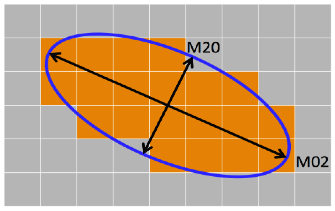
\includegraphics[width=.35\linewidth]{m02&m20.png}
\caption{Schematische Darstellung eines \textit{Clusters}. Die Ellipsenhalbachsen $M_{20}$ und $M_{02}$ definieren eine Ellipse, die alle orange markierten Zellen, die zu einem \textit{Cluster} in einem Kalorimeter mit quadratischen Zellen gehören, umfasst.
[\cite{thesis:Adrian}]}
\label{fig:$M_{20}$}
\end{figure}
Abbildung \ref{fig:$M_{20}$} zeigt eine schematische Darstellung eines \textit{Clusters}.
Alle orange eingefärbten Zellen gehören dabei zu dem \textit{Cluster}.
Die eingezeichnete Ellipse, beziehungsweise ihre Halbachsen $M_{02}$ und $M_{20}$, helfen dabei, das \textit{Cluster} zu parametrisieren.
Die Form eines \textit{Clusters} und damit die Größe von $M_{02}$ und $M_{20}$ unterscheidet sich abhängig davon, ob das \textit{Cluster} durch ein Photon entstanden ist oder nicht.
Dadurch kann $M_{02}$ benutzt werden, um \textit{Cluster,} die durch Photonen entstanden sind, zu identifizieren.
Für $M_{02}$ gilt:
\begin{align} 
M_{02} = \frac{1}{2}\sum_{i}E_{i}(x_{i}^{2}+y_{i}^{2})+\sqrt{\frac{1}{4}\sum_{i}\left(x_{i}^{2}+y_{i}^{2}\right)^{2}+\left(\sum_{i}E_{i}x_{i}y_{i}\right)}
\end{align}
Wobei $E_{i}$ für die Energie einer Zelle und $x_{i}$ und $y_{i}$ für die relative Position einer Zelle zur Startzelle steht.
\newline
Nachdem die Grundlagen zur Theorie und dem Experiment erklärt wurden, wird im nächsten Abschnitt die Analyse erläutert.
Dazu wird zunächst die Auswahl der Daten, die in dieser Arbeit benutzt werden, aufgeführt.